\documentclass[paper=a4, fontsize=11pt]{scrartcl} % KOMA-article class

%-------------------------------------------------
%   THEMES, PACKAGES, CUSTOM COMMANDS
%-------------------------------------------------
\usepackage{blindtext}
\usepackage[english]{babel}                             % English language/hyphenation
\usepackage[protrusion=true,expansion=true]{microtype}  % Better typography
\usepackage{amsmath,amsfonts,amsthm}                    % Math packages
\usepackage[pdftex]{graphicx}                           % Enable pdflatex
\usepackage[export]{adjustbox}
\usepackage[svgnames]{xcolor}                           % Enabling colors by their 'svgnames'
\usepackage[hang, small,labelfont=bf,up,textfont=it,up]{caption} % Custom captions under/above floats
\usepackage{subcaption}
\usepackage{caption}
\usepackage{epstopdf}       % Converts .eps to .pdf
%\usepackage{subfig}         % Subfigures
\usepackage{booktabs}       % Nicer tables
\usepackage{fix-cm}         % Custom fontsizes
\usepackage{listings}
\usepackage{soul}
\usepackage{float}

\usepackage{hyperref}

\usepackage[foot=30pt,margin=1in]{geometry}

\usepackage{listings}
\definecolor{mygreen}{rgb}{0,0.6,0}
\definecolor{mygray}{rgb}{0.5,0.5,0.5}
\definecolor{mymauve}{rgb}{0.58,0,0.82}
\lstset{ %
    backgroundcolor=\color{white},   % choose the background color; you must add \usepackage{color} or \usepackage{xcolor}
    basicstyle=\footnotesize,        % the size of the fonts that are used for the code
    breakatwhitespace=false,         % sets if automatic breaks should only happen at whitespace
    breaklines=true,                 % sets automatic line breaking
    captionpos=b,                    % sets the caption-position to bottom
    commentstyle=\color{mygreen},    % comment style
    deletekeywords={...},            % if you want to delete keywords from the given language
    escapeinside={\%*}{*)},          % if you want to add LaTeX within your code
    extendedchars=true,              % lets you use non-ASCII characters; for 8-bits encodings only, does not work with UTF-8
    frame=single,                    % adds a frame around the code
    keepspaces=true,                 % keeps spaces in text, useful for keeping indentation of code (possibly needs columns=flexible)
    keywordstyle=\color{blue},       % keyword style
    language=Python,                 % the language of the code
    morekeywords={*,...},            % if you want to add more keywords to the set
    numbers=left,                    % where to put the line-numbers; possible values are (none, left, right)
    numbersep=5pt,                   % how far the line-numbers are from the code
    numberstyle=\tiny\color{mygray}, % the style that is used for the line-numbers
    rulecolor=\color{black},         % if not set, the frame-color may be changed on line-breaks within not-black text (e.g. comments (green here))
    showspaces=false,                % show spaces everywhere adding particular underscores; it overrides 'showstringspaces'
    showstringspaces=false,          % underline spaces within strings only
    showtabs=false,                  % show tabs within strings adding particular underscores
    stepnumber=2,                    % the step between two line-numbers. If it's 1, each line will be numbered
    stringstyle=\color{mymauve},     % string literal style
    tabsize=3,                       % sets default tabsize to 2 spaces
    title=\lstname                   % show the filename of files included with \lstinputlisting; also try caption instead of title
}

% Custom sectioning (sectsty package)
\usepackage{sectsty}
\allsectionsfont{
    \usefont{OT1}{phv}{b}{n}    % bch-b-n: CharterBT-Bold font
}
\sectionfont{
    \usefont{OT1}{phv}{b}{n}
}

% Custom colors
\definecolor{brsugrey}{rgb}{0.9, 0.9, 0.9}
\definecolor{brsublue}{rgb}{0, 0.594, 0.949}

%
\newcommand{\upperRomannumeral}[1]{\uppercase\expandafter{\romannumeral#1}}

% Creating an initial of the very first character of the content
\usepackage{lettrine}
\newcommand{\initial}[1]{%
    \lettrine[lines=3,lhang=0.3,nindent=0em]{
        \color{brsublue}
        {\textsf{#1}}}{}}

%-------------------------------------------------
%   COMMON INFO
%-------------------------------------------------
\newcommand{\hmwkTitle}{MNIST Digit Classification Report}
\newcommand{\hmwkDueDate}{Monday, January 19, 2017}
\newcommand{\hmwkClass}{Scientific Evaluation and Experimentation}
\newcommand{\hmwkClassShort}{SEE WS2016}
\newcommand{\hmwkAuthorFullName}{Minh H. Nguyen \& Bach D. Ha}
\newcommand{\hmwkAuthorLastName}{Nguyen \& Ha}
\newcommand{\hmwkAuthorEmail}{minh.nguyen@smail.inf.h-brs.de\\
                              bach.ha@smail.inf.h-brs.de}
\newcommand{\hmwkAuthorInstitute}{BRS University of Applied Sciences}

%-------------------------------------------------
%   HEADERS & FOOTERS
%-------------------------------------------------
\usepackage{fancyhdr}
\pagestyle{fancy}
\usepackage{lastpage}
% Header (empty)
\lhead{}
\chead{}
\rhead{}
% Footer (you may change this to your own needs)
\lfoot{\footnotesize
    \texttt{\hmwkClassShort} ~
    \textbullet ~ \hmwkAuthorLastName ~
    \textbullet ~ \hmwkTitle}
\cfoot{}
\rfoot{\footnotesize page \thepage\ of \pageref{LastPage}}  % "Page 1 of 2"
\renewcommand{\headrulewidth}{0.0pt}
\renewcommand{\footrulewidth}{0.4pt}

%-------------------------------------------------
%   TITLE & AUTHOR
%-------------------------------------------------
\usepackage{titling}

\newcommand{\HorRule}{\color{brsublue}% Creating a horizontal rule
    \rule{\linewidth}{1pt}%
    \color{black}
}

% Title
\pretitle{
    \vspace{-30pt}
    \begin{flushleft}
        \HorRule
        \fontsize{22}{22} \usefont{OT1}{phv}{b}{n} \color{gray} \selectfont
}
\title{\hmwkClass \\
       \hmwkTitle}
\posttitle{
    \par
    \end{flushleft}
    \vskip 0.5em
}

% Author
\preauthor{
    \begin{flushleft}
        \large \lineskip 0.25em
        \usefont{OT1}{phv}{b}{sl} \color{brsublue}}

\author{\hmwkAuthorFullName}

\postauthor{
        \footnotesize
        \usefont{OT1}{phv}{m}{sl} \color{Black}
        \\\hmwkAuthorInstitute
        \\\hmwkAuthorEmail
        \par
    \end{flushleft}
    \HorRule}

% Date
\date{\hmwkDueDate}

%-------------------------------------------------
%   BEGIN
%-------------------------------------------------
\begin{document}
    \maketitle
    \thispagestyle{fancy} % Enabling the custom headers/footers for the first page

\section*{Convolutional Neural Networks VS Support Vector Machine}
    \subsection*{Machine learner}	
   	\begin{itemize}
   		\item CNN: 
   		\begin{itemize}
   			\item Simple model with the following overall architecture
   			\[Convolution - MaxPooling - FullyConnect - FullyConnect\] 
   			\item Implementation: Keras: 10-15 lines of code, must explicitly set at least 10 parameters.
   		\end{itemize}
   		\item SVM: 
   		\begin{itemize}
   			\item Multi-class SVM with Rbf kernel.
   			\item Implementation: Scikit learn: 3-5 lines of code. No need for explicitly setting any hyper-parameters, default value is already good.
   		\end{itemize}
  	\end{itemize}

    \subsection*{Training}
	\begin{itemize}
		\item General: 67\% of the data set is used for training. The rest is for testing.
		\item CNN: Trained for 150 epochs, each epoch last around 160 seconds
		\item SVM: Training is done in 430 seconds in total.
	\end{itemize}


    \begin{figure}[H]
        \begin{center}
            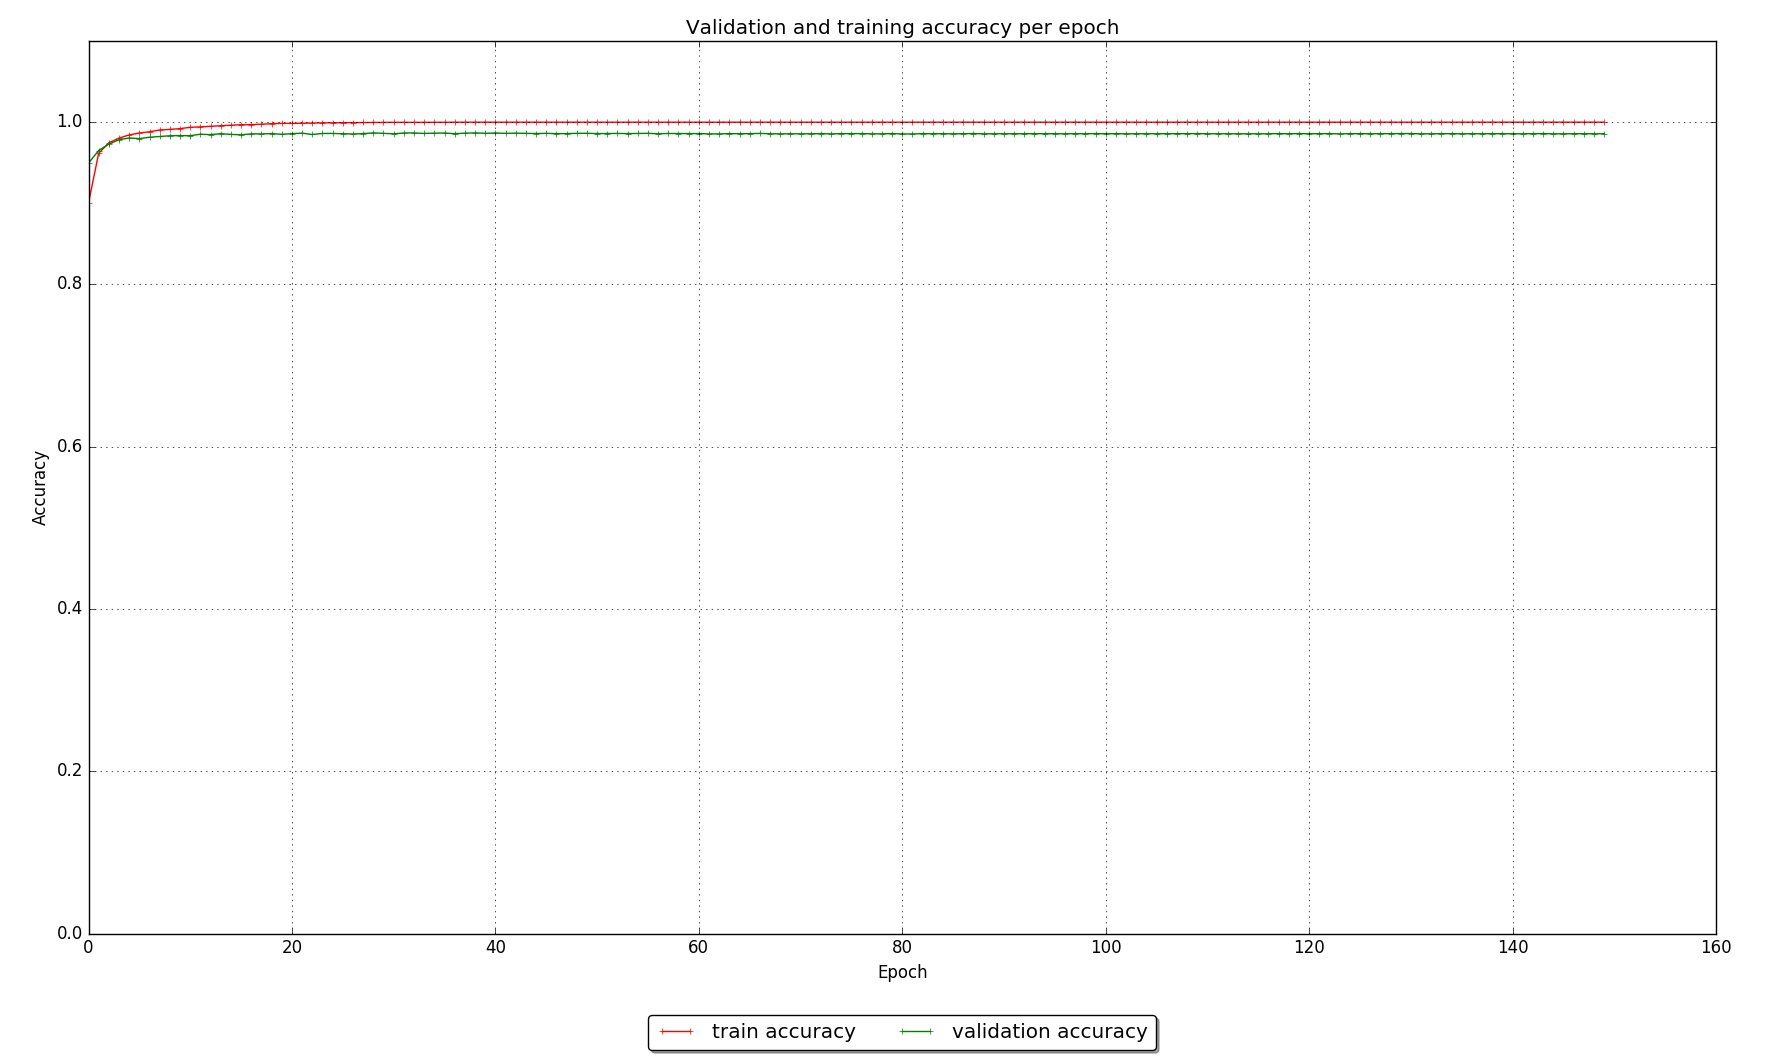
\includegraphics[width=1.0\linewidth]{images/mnist_training_log.png}
            \caption{Accuracy per epoch when training CNN}
            \label{fig:train}
        \end{center}
    \end{figure}
    
    \subsection*{Performance}
    	\begin{itemize}
    		\item CNN: 
    		\begin{itemize}
    			\item Accuracy after 1st epoch: 0.95
    			\item Accuracy after 25th epoch: 0.986
    			\item No overfitting in later epochs
    		\end{itemize}
    		\item SVM: 
    		\begin{itemize}
    			\item Accuracy: 0.93
    		\end{itemize}
   		\end{itemize}
   		
    \begin{figure}[H]
        \begin{center}
            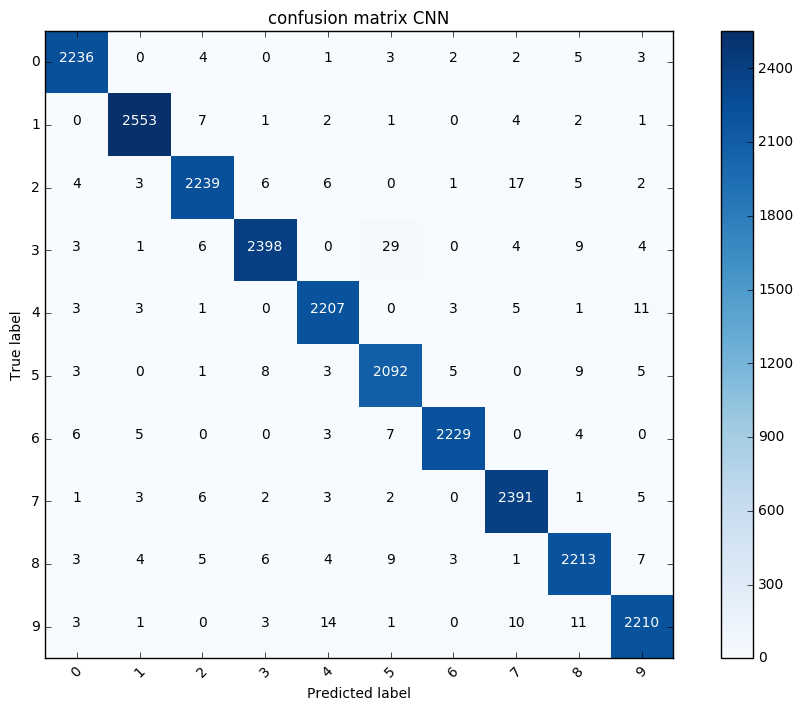
\includegraphics[width=1.0\linewidth]{images/confusion_matrix_CNN}
            \caption{Confusion matrix - CNN - After 150 epochs}
            \label{fig:con_mat_CNN}
        \end{center}
    \end{figure}
    
    \begin{figure}[H]
        \begin{center}
            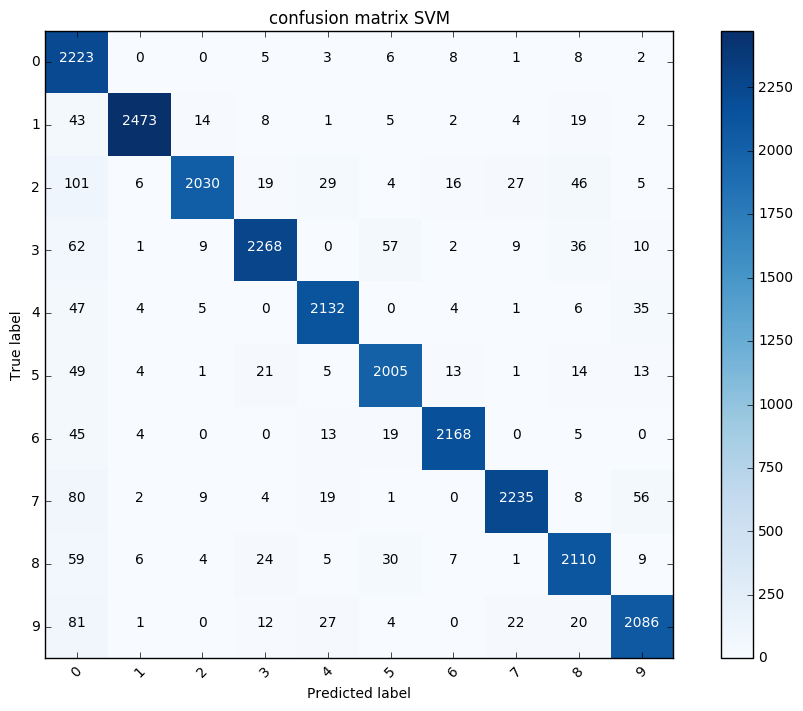
\includegraphics[width=1.0\linewidth]{images/confusion_matrix_SVM}
            \caption{Confusion matrix - SVM}
            \label{fig:con_mat_SVM}
        \end{center}
    \end{figure} 
   		
   		
   	\subsection*{Conclusion}
	With similar amount of training time, 3 epochs for CNN, the performance of both CNN and SVM are actually similar. However, CNN's accuracy can be further improved with more training, while SVM's accuracy cannot be improved further. So it can be say that CNN beats SVM in term that CNN's final accuracy limit is higher. On the other hand, SVM is much easier to use than CNN, because users do not even have to set a single hyper-parameter for it to work well.
    
\end{document}
